% 旋转构造 引入/例1：正方形 ABCD 内一点 P, PA=1, PB=2, PC=3
\documentclass[tikz,border=4pt]{standalone}
\usepackage{ctex}
\usepackage{amsmath}
\usetikzlibrary{calc}
\begin{document}
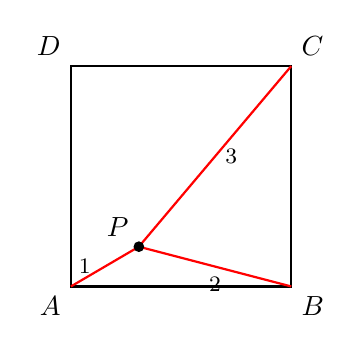
\begin{tikzpicture}[scale=1.0, thick]
  % 正方形边长足够大: 设 边长 a. 选 A=(0,0) B=(a,0) C=(a,a) D=(0,a)
  % P 满足 PA=1, PB=2, PC=3 -> 唯一确定 a 和 P 位置
  % 通过约束: P=(x,y), x²+y²=1, (x-a)²+y²=4, (x-a)²+(y-a)²=9
  % 第二式 - 第一式: -2ax+a²=3 -> a² - 2ax = 3
  % 第三式 - 第二式: -2ay+a²=5 -> a² - 2ay = 5
  % 又 x²+y²=1
  % 设 a≈2.4 (常见值)... 直接计算: 由前两式 x = (a²-3)/(2a), y = (a²-5)/(2a)
  % 代入 x²+y²=1: [(a²-3)²+(a²-5)²]/(4a²) = 1
  % (a²-3)²+(a²-5)² = 4a²
  % 展开: a⁴-6a²+9 + a⁴-10a²+25 = 4a², 2a⁴-16a²+34=4a², 2a⁴-20a²+34=0
  % a⁴-10a²+17=0, a²=(10±√(100-68))/2=(10±√32)/2=5±2√2
  % a²=5+2√2 ≈ 7.828, a≈2.798
  % x = (a²-3)/(2a) = (2+2√2)/(2a) = (1+√2)/a ≈ 2.414/2.798 ≈ 0.863
  % y = (a²-5)/(2a) = 2√2/(2a) = √2/a ≈ 1.414/2.798 ≈ 0.505
  \def\a{2.798}
  \coordinate (A) at (0,0);
  \coordinate (B) at (\a,0);
  \coordinate (C) at (\a,\a);
  \coordinate (D) at (0,\a);
  \coordinate (P) at (0.863, 0.505);
  \draw (A)--(B)--(C)--(D)--cycle;
  \draw[red] (A)--(P);
  \draw[red] (B)--(P);
  \draw[red] (C)--(P);
  \filldraw (P) circle (1.5pt);
  \node[below left] at (A) {$A$};
  \node[below right] at (B) {$B$};
  \node[above right] at (C) {$C$};
  \node[above left] at (D) {$D$};
  \node[above left] at (P) {$P$};
  \node[left] at ($(A)!0.5!(P) + (-0.05,0)$) {\footnotesize $1$};
  \node[below] at ($(B)!0.5!(P)$) {\footnotesize $2$};
  \node[right] at ($(C)!0.5!(P)$) {\footnotesize $3$};
\end{tikzpicture}
\end{document}
